\documentclass[12pt]{exam}

\usepackage{amssymb, amsmath, amsthm, mathrsfs, multicol, graphicx}
\usepackage{tikz}
\usepackage{array}


 \def\d{\displaystyle}
\def\?{\reflectbox{?}}
\def\b#1{\mathbf{#1}}
\def\f#1{\mathfrak #1}
\def\c#1{\mathcal #1}
\def\s#1{\mathscr #1}
\def\r#1{\mathrm{#1}}
\def\N{\mathbb N}
\def\Z{\mathbb Z}
\def\Q{\mathbb Q}
\def\R{\mathbb R}
\def\C{\mathbb C}
\def\F{\mathbb F}
\def\A{\mathbb A}
\def\X{\mathbb X}
\def\E{\mathbb E}
\def\O{\mathbb O}
\def\U{\mathcal U}
\def\pow{\mathcal P}
\def\inv{^{-1}}
\def\nrml{\triangleleft}
\def\st{:}
\def\~{\widetilde}
\def\rem{\mathcal R}
\def\sigalg{$\sigma$-algebra }
\def\Gal{\mbox{Gal}}
\def\iff{\leftrightarrow}
\def\Iff{\Leftrightarrow}
\def\land{\wedge}
\def\And{\bigwedge}
\def\AAnd{\d\bigwedge\mkern-18mu\bigwedge}
\def\Vee{\bigvee}
\def\VVee{\d\Vee\mkern-18mu\Vee}
\def\imp{\rightarrow}
\def\Imp{\Rightarrow}
\def\Fi{\Leftarrow}

%\def\={\equiv}
\def\var{\mbox{var}}
\def\mod{\mbox{Mod}}
\def\Th{\mbox{Th}}
\def\sat{\mbox{Sat}}
\def\con{\mbox{Con}}
\def\bmodels{=\joinrel\mathrel|}
\def\iffmodels{\bmodels\models}
\def\dbland{\bigwedge \!\!\bigwedge}
\def\dom{\mbox{dom}}
\def\rng{\mbox{range}}
\DeclareMathOperator{\wgt}{wgt}


\def\bar{\overline}


\newcommand{\vtx}[2]{node[fill,circle,inner sep=0pt, minimum size=4pt,label=#1:#2]{}}
\newcommand{\va}[1]{\vtx{above}{#1}}
\newcommand{\vb}[1]{\vtx{below}{#1}}
\newcommand{\vr}[1]{\vtx{right}{#1}}
\newcommand{\vl}[1]{\vtx{left}{#1}}
\renewcommand{\v}{\vtx{above}{}}

\def\circleA{(-.5,0) circle (1)}
\def\circleAlabel{(-1.5,.6) node[above]{$A$}}
\def\circleB{(.5,0) circle (1)}
\def\circleBlabel{(1.5,.6) node[above]{$B$}}
\def\circleC{(0,-1) circle (1)}
\def\circleClabel{(.5,-2) node[right]{$C$}}
\def\twosetbox{(-2,-1.4) rectangle (2,1.4)}
\def\threesetbox{(-2.5,-2.4) rectangle (2.5,1.4)}
\newcommand{\twoline}[2]{\begin{pmatrix}#1 \\ #2 \end{pmatrix}}


\def\circleA{(-.5,0) circle (1)}
\def\circleAlabel{(-1.5,.6) node[above]{$A$}}
\def\circleB{(.5,0) circle (1)}
\def\circleBlabel{(1.5,.6) node[above]{$B$}}
\def\circleC{(0,-1) circle (1)}
\def\circleClabel{(.5,-2) node[right]{$C$}}
\def\twosetbox{(-2,-1.5) rectangle (2,1.5)}
\def\threesetbox{(-2,-2.5) rectangle (2,1.5)}

%\pointname{pts}
\pointsinmargin
\marginpointname{pts}
\marginbonuspointname{bn-pts}
\addpoints
\pagestyle{head}
\printanswers

\firstpageheader{Math 228}{\bf Homework 9 Solutions}{Due: Wednesday, October 31}


\begin{document}
% \noindent \textbf{Instructions}: Same rules as usual.  Turn in solutions on separate pages, and do not consult the internet.

\begin{questions}
	% \question[6] Write out the first 5 terms (starting with $a_0$) of each of the sequences described below.  Then give either a closed formula or a recursive definition for the sequence (whichever is NOT given in the problem).
	% \begin{parts}
	% \part $a_n = \frac{1}{2}(n^2 + n)$.
	% \begin{solution}
	% $a_0 = 0$, $a_1 = 1$, $a_2 = 3$, $a_3 = 6$ $a_4 = 10$. The sequence was described by a closed formula.  These are the triangular numbers.  A recursive definition is: $a_n = a_{n-1} + n$ with $a_0 = 0$.
	% \end{solution}
	% 
	% \part $a_n = 2a_{n-1} - a_{n-2}$ with $a_0 = 0$ and $a_1 = 1$.
	% \begin{solution}
	% This is a recursive definition.  We continue $a_2 = 2$, $a_3 = 3$, $a_4 = 4$, $a_5 = 5$, and so on.  A closed formula is $a_n = n$.
	% \end{solution}
	% 
	% \part $a_n = na_{n-1}$ with $a_0 = 1$.
	% \begin{solution}
	% We have $a_0 = 1$, $a_1 = 1$, $a_2 = 2$, $a_3 = 6$, $a_4 = 24$, $a_5 = 120$, and so on.  The closed formula is $a_n = n!$.
	% \end{solution}
	% \end{parts}
	% 
	% \question[8] For each sequence given below, find a closed formula for $a_n$, the $n$th term of the sequence (assume the first terms are $a_0$) by relating it to another sequence for which you already know the formula.  In each case, briefly say how you got your answers.
	% \begin{parts}
	% 	\part 4, 5, 7, 11, 19, 35, \ldots
	% 	\begin{solution}
	% 		If we subtract 3 from each term, we get $1, 2, 4, 8, 16, 32, \ldots$, which are the powers of 2.  So we must shift this sequence up by 3 to get our sequence.  Thus
	% 		\[a_n = 2^n + 3\]
	% 	\end{solution}
	% 
	% 	\part 0, 3, 8, 15, 24, 35, \ldots
	% 	\begin{solution}
	% 		Add 1 to each term - we get $1, 4, 9, 16, 25, 36, \ldots$, the square numbers.  So maybe our sequence as formula $a_n = n^2 - 1$.  Does this work?  $a_3 = 8$.  That is a term of our sequence, but it should be $a_2$.  So we want
	% 		\[a_n = (n+1)^2 - 1\]
	% 	\end{solution}
	% 
	% 	\part 6, 12, 20, 30, 42, \ldots
	% 	\begin{solution}
	% 		Each term is even, so let's see what happens when we divide by 2: we get $3, 6, 10, 15, 21,\ldots$.  These are the triangle numbers, but starting at $T_2$.  We know $T_n = \frac{n(n+1)}{2}$. We want $a_0 = 2T_2$, $a_1 = 2T_3$, and so on.  In general, $a_n = 2T_{n+2}$, so
	% 		\[a_n = (n+2)(n+3)\]
	% 		(This is like a shift by 2 units to the left and a stretch by a factor of 2.)
	% 	\end{solution}
	% 
	% 	\part 0, 2, 7, 15, 26, 40, 57, \ldots (Hint: this is the \emph{sum} of two well known sequences.)
	% 	\begin{solution}
	% 		How far off from triangular number are these?  The triangular numbers (starting with $T_0$) are $0, 1, 3, 6, 10, 15, 21, \ldots$.  The given sequence differs from this by $0, 1, 4, 9, 16, 25, 36, \ldots$ the square numbers!  Thus
	% 		\[a_n = \frac{n(n+1)}{2} + n^2\]
	% 	\end{solution}
	% \end{parts}




	\question[8] Starting with any rectangle, we can create a new, larger rectangle by attaching a square to the longer side.  For example, if we start with a $2\times 5$ rectangle, we would glue on a $5\times 5 $ square, forming a $5 \times 7$ rectangle:

	\begin{center}
		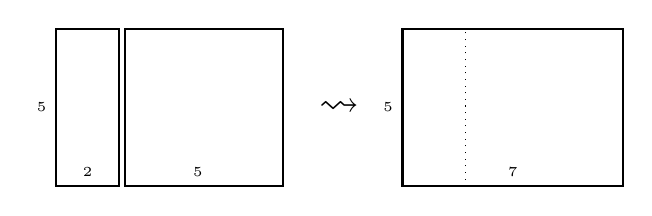
\begin{tikzpicture}[scale=.4]
			\draw[thick] (0,0) rectangle (2,5);
			\draw[thick] (2.2,0) rectangle (7.2,5);
			\draw (0,2.5) node[left]{\tiny 5} (1,0) node[above]{\tiny 2} (4.5,0) node[above]{\tiny 5};
			\draw (9,2.5) node{\Large $\rightsquigarrow$};
			\draw[thick] (11,0) rectangle (18,5);
			\draw[dotted] (13,0) -- (13,5);
			\draw (11,2.5) node[left]{\tiny 5}  (14.5,0) node[above]{\tiny 7};
		\end{tikzpicture}
	\end{center}

The next rectangle would be formed by attaching a $7\times 7$ square to the \emph{top or bottom} of the $5 \times 7$ rectangle.
	\begin{parts}
		\part Create a sequence of rectangles using this rule starting with a $1\times 2$ rectangle.  Then write out the sequence of \emph{perimeters} for the rectangles (the first term of the sequence would be 6, since the perimeter of a $1\times 2$ rectangle is 6, the next term would be 10).
		\begin{solution}
			The rectangles are $1 \times 2$, $2 \times 3$, $3 \times 5$, $5 \times 8$, $8 \times 13$, and so on.  The sequence of perimeters is \[6, 10, 16, 26, 42, \ldots\]
		\end{solution}

		\part Repeat the above part this time starting with a $1 \times 3$ rectangle.
		\begin{solution}
			The sequence of rectangles have dimensions $1\times 3$, $3 \times 4$, $4 \times 7$, $7 \times 11$, $11\times 18$, and so on.  The sequence of perimeters is \[8, 14, 22, 36, 58, \ldots\]
		\end{solution}

		\part Find recursive definitions for each of the sequences of perimeters you found in parts (a) and (b).  Don't forget to give the initial conditions as well.
		\begin{solution}
			For the sequence from (a), the recursive formula is $a_1 = 6$, $a_2 = 10$, and $a_n = a_{n-1} + a_{n-2}$.

			For the sequence from (b), the recursive formula is $a_1 = 8$, $a_2 = 14$, and $a_n = a_{n-1} + a_{n-2}$.

			Notice that both sequence have the same rule for getting terms from the previous ones, it is just the initial conditions that are different.
		\end{solution}

		\part Are the sequences arithmetic?  Geometric?  If not, are they {\em close} to being either of these (i.e., are the differences or ratios {\em almost} constant)?  Write down the sequences of differences and sequences of ratios and explain anything interesting you find.
		\begin{solution}
			The sequences are not arithmetic because the differences between terms is not constant.  Similarly the ratio between terms is not constant, so the sequences are not geometric either.

			However, look at the ratio between terms: $10/6 \approx 1.66$, $16/10 = 1.6$, $26/16 \approx 1.625$, $42/26 \approx 1.61$, \ldots.  In fact, the ratio between terms of the second sequence also floats around this same number.

			That number (and in fact, the limit of the ratios of either sequence as the terms increase) is $\frac{1 + \sqrt{5}}{2} \approx 1.618$, also known as the golden ratio.
			\end{solution}
	\end{parts}


	\question[4] The Skittles machine at King Soopers is \emph{magic}.  The first time you put a coin in, you get 5 Skittles.  Every time after that, you get 3 more skittles than the last time.
	\begin{parts}
		\part How many Skittles will the machine dispense on the $n$th coin?
		\begin{solution}
			A recursive formula for this sequence is $a_n = a_{n-1} + 3$, which comes from the description in the problem.  So this is an arithmetic sequence: $a_n = 2 + 3n$ for $n \ge 1$.  
		\end{solution}
		\part How many Skittles will the machine have dispensed all together after the $n$th coin?  Show your work.
		\begin{solution}
			We are looking for the sequence of partial sums:
			
			\centerline{
			\begin{tabular}{lrcl}
				& $S_n$ & $=$ & $5 + 8 + 11 + \cdots + (2+3n)$ \\
				\textsc{\scriptsize add}~~~ & $S_n$ & $=$ & $(2+3n) + \cdots + 11 + 8 + 5$\\ \hline
				 & $2S_n$ & $=$ & $(7+3n) + \cdots + (7+3n)$
			\end{tabular}
			}
			
			So $S_n = \frac{n(7+3n)}{2}$.
		\end{solution}
	\end{parts}

	\question[4] Not to be outdone, Safeway has procured a magic Runts machine, that dispenses 3 candies for the first coin, and every time after that, twice as many candies as the previous time.
	\begin{parts}
		\part How many Runts will the machine dispense on the $n$th coin?
		\begin{solution}
			Recursively, we see the formula will be $a_n = 2a_{n-1}$ with $a_1 = 3$.  This is a geometic sequence.  The closed formula is then $a_n = 3\cdot 2^{n-1}$.
		\end{solution}
		\part How many Runts will the machine have dispensed all together after the $n$th coin?  Show your work.
		\begin{solution}
			Again we are looking for a sequence of partial sums:
			
			\centerline{
			\begin{tabular}{lrcll}
				& $S_n$ & $=$ & $3 + $ & $6 + 12 + \cdots + 3\cdot 2^{n-1}$ \\
			\textsc{\tiny subtract}	~~	& $2S_n$ & $=$ & & $3+6 + 12 + \cdots + 3\cdot 2^{n}$ \\ \hline
			& $(1-2)S_n$ & $=$ & $3 - 3\cdot 2^{n}$
			\end{tabular}
			}
			
			So $S_n = \frac{3-3\cdot 2^n}{1-2} = 3\cdot 2^n - 3$.
		\end{solution}
		
	\end{parts}

	\question Fibonacci's Grocers has a machine that dispenses Smarties candies.  The first two times a coin is inserted, only one candy is dispensed.  After that, the number of candies is the sum of the previous two times.  As in the previous two problems, you would like to find an expression for the total number of candies dispensed after the $n$th coin.
	\begin{parts}
		\part[3] Carefully explain why neither \emph{reverse and add} nor \emph{multiple-shift-subtract} (the methods from the previous two problems) work to find this sum.
		\begin{solution}
			We cannot reverse and add, because the difference between terms is not constant.  For example, if we did the 5th partial sum, we would be looking at $1+1+2+3+5$.  Reversed: $5+3+2+1+1$.  Adding corresponding elements (straight down) gives $6 + 4 + 4 + 4 + 6$, so since this is not the sum of one constant, we cannot simplify any further.
			
			You also cannot multiply-shift-subtract since the ratio between terms is not constant.  There is nothing you can multiply each term by to get the next terms, so there is no way to have most of the terms cancel out.
		\end{solution}
		\part[2] Write out the sequence of partial sums (i.e., the number of candies dispensed after the $n$th coin for different values of $n$) and conjecture a formula for the $n$th term of the sequence, in terms of Fibonacci numbers.
		\begin{solution}
			The sequence of partial sums is $1, 2, 4, 7, 12, 20, \ldots$.  These appear to be one less than a Fibonacci number.  So we guess $S_n = F_{n+2} - 1$
		\end{solution}
		\part[3] Prove your formula is correct using mathematical induction.
		\begin{solution}
			Let $P(n)$ be the statement $F_1 + F_2 + F_3 + \cdots + F_n = F_{n+2} - 1$.  
			
			Base case.  $P(1)$ is true because $F_1 = 1$ and $F_3-1 = 2-1 = 1$.
			
			Inductive case.  Assume $P(k)$ is true.  That is, we can add up the first $k$ Fibonacci numbers and get $F_{k+2} - 1$.  To verify $P(k+1)$, consider the sum of the first $k+1$ Fibonacci numbers.  We must add up the first $k$ Fibonacci numbers, plus the $F_{k+1}$.  The sum of the first $k$ Fibonacci numbers is $F_{k+2} - 1$ so the total sum will be 
			\[F_1 + F_2 + \cdots + F_{k+1} = F_{k+2} - 1 + F_{k+1}\]
			But using the recurrence relation for the Fibonacci numbers, we see that the right hand side is just $F_{k+3} - 1$, which is what we wanted to show.
			
			Therefore, by the principle of mathematical induction, $P(n)$ is true for all $n$.
		\end{solution}
	\end{parts}

	\question[6]\label{diamonds} If you were to shade in a $n\times n$ square on graph paper, you could do it the boring way (with sides parallel to the edge of the paper) or the interesting way, as illustrated below:


	\begin{center}
	  \begin{tabular}{m{2cm}m{3cm}m{4cm}m{3cm}}
	  \begin{tikzpicture}[scale=0.4]
	    \draw (0,0) rectangle (1,1);
	  \end{tikzpicture}
	  &
	  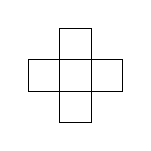
\begin{tikzpicture}[scale=0.4]
	    \draw (-1,0) rectangle (2,1) (0,-1) rectangle (1,2);
	  \end{tikzpicture}
	  &
	  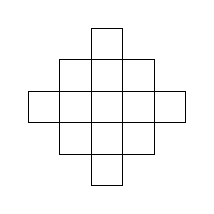
\begin{tikzpicture}[scale=0.4]
	    \draw (-2,0) rectangle (3,1) (0,-2) rectangle (1,3) (-1,-1) rectangle (2,2);
	  \end{tikzpicture}
	  &
	  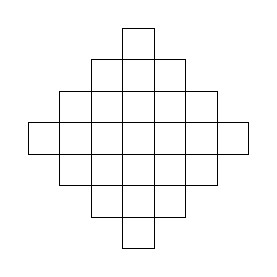
\begin{tikzpicture}[scale=0.4]
	    \draw (-3,0) rectangle (4,1) (-2,-1) rectangle (3,2) (-1,-2) rectangle (2,3) (0,-3) rectangle (1,4);
	  \end{tikzpicture}
	\end{tabular}
	\end{center}

	The interesting thing here, is that a $3\times 3$ square now has area 13.  Our goal is the find a formula for the area of a $n \times n$ (diagonal) square.

	\begin{parts}
	  \part Write out the first few terms of the sequence of areas (assume $a_1 = 1$, $a_2 = 5$, etc).  Is the sequence arithmetic or geometric?  If not, is it the sequence of partial sums of an arithmetic or geometric sequence?  Explain why your answer is correct, referring to the diagonal squares.

	  \begin{solution}
	    The sequence is $1, 5, 13, 25, 41, 61, \ldots$.  This is not arithmetic
		  (since $5-1 = 4$ but $13-5 = 8$).  It is also not geometric (since $5/1 = 5$ but $13/5 = 2.6$).  To recognize whether the sequence is a sequence of partial sums, we look at the differences.  The sequence of differences is $4, 8, 12, 16, 20, \ldots$.  This {\em is} an arithmetic sequence.  So we see that
		  \[a_1 = 1\]
		  \[a_2 = 1+4\]
		  \[a_3 = 1+4+8\]
		  \[a_4 = 1+4+8+12\]
		  \[a_n = 1 + \sum_{k = 1}^n 4(k-1)\]
	  \end{solution}

	  \part Use your results from part (a) to find a closed formula for the sequence.  Show your work.  Note, while there are lots of ways to find a closed formula here, you should use partial sums specifically.
	  \begin{solution}
	    We have $a_n = 1 + 4 + 8 + \cdots + 4(n-1)$.  If we reverse these and add corresponding terms (not including the 1) we get
	    \[2a_n = 2 + (4n) + (4n) + (4n) + \cdots + (4n)\]
	    On the right hand side of the equation we have the sum of $n-1$ copies of $(4n)$ so we get
	    \[2a_n = 2 + (n-1)(4n)\]
	    or \[a_n = 2n^2 - 2n + 1\]
	  \end{solution}
	\end{parts}
	
	\bonusquestion[4] Bonus: For the sequence in question \ref{diamonds}, find the closed formula in as many interesting ways as you can.  Each unique explanation gets 1 point.

	\begin{solution}
	  There are lots of interesting things you can do here.  From what we have done with sequences, you could notice that the second differences are constant, so you know that the closed formula will be quadratic.  You could then use polynomial fitting, or simply compare the sequence to $n^2$ to find the pattern.  More inventive solutions include:
	  \begin{enumerate}
	    \item Look along the diagonals.  The $n$th figure will have $n$ diagonals of $n$ squares, and $n-1$ diagonals of $n-1$ squares.  Thus all together, the number of squares is $n^2 + (n-1)^2$.
	    \item If you count the number of squares in each row starting at the top, you will have $1, 3, 5, \ldots, 2n-3, 2n-1, 2n-3, \ldots, 3, 1$.  So we can think of the total number of squares as being the sum of the first $n$ odd numbers (counting up) plus the sum of the first $n-1$ odd numbers (counting down).  But the sum of the first $n$ odd numbers is $n^2$, so again we find the total number of squares to be $n^2 + (n-1)^2$.
	    \item Enclose the figure in a larger square with dimensions $2n-1 \times 2n-1$.  Then look at what part of that square you don't want.  You have 4 triangles you must remove.  The $n$th figure requires removing a triangle with base $n-1$ on each corner, so we must remove $4T_{n-1}$, where $T_n = \frac{n(n+1)}{2}$ is the $n$th triangular number.  Thus the total number of squares in the figure is
	    \[(2n-1)^2 - 4\frac{(n-1)n}{2}.\]
	  \end{enumerate}
	\end{solution}

\end{questions}




\end{document}
